\documentclass[letterpaper,11pt]{article}
\usepackage[margin=1in]{geometry}
\usepackage{natbib}
% \bibliographystyle{unsrtnat}
\usepackage{tabularx} % extra features for tabular environment
\usepackage{amsmath}  % improve math presentation
\usepackage{graphicx} % takes care of graphic including machinery
% \usepackage{cite} % takes care of citations
\usepackage[final]{hyperref} % adds hyper links inside the generated pdf file
\usepackage{longtable}
\usepackage{xcolor}

% ------------------------------------------------------------------------
\newcommand{\myCheckBox}{\CheckBox[width=0.8em,bordercolor={0.65 0.79 0.94},height=0.8em]}
\newcommand{\dC}        {$^\circ$C}
\renewcommand{\arraystretch}{1.3}

% ------------------------------------------------------------------------

\begin{document}

\title{\textbf{SLArchetto Operation Procedure}}
\author{Yun-Tse Tsai}
\date{\today}

\maketitle

%-------------------------------------------------------------------

\underline{General steps:}
\begin{enumerate}
\setlength\itemsep{-0.2em}
\item Precool the LAr filter first.  During the precooling, vent to the venting line, 
but not to the SLArchetto vessel.  This takes about 1 hour and we stop precooling when the
temperature in the LAr filter is {\color{orange}? {\dC}}.
\item Fill the SLArchetto vessel, monitor the LArPix noise during the filling.
\item After LAr reaches the desired level, take pedestal data with LArPix.
\item Turn off LArPix and ramp up the high voltage.
\item Take pedestal data, set the trigger threshold of LArPix.  Start data taking.
\end{enumerate}  

\underline{Safety:}
\begin{itemize}
\setlength\itemsep{-0.2em}
\item All the doors of the LNTF hut have to be open.
\item The intake fan has to be turned on.
\item The oxygen deficiency sensor and monitor (ODM) have to be checked.
\item The pressure in the LAr filter must not exceed 150~psi.  The pressure is shown on PG3.
\item The pressure in the SLArchetto vessel must not exceed 10~psig.  The cracking pressure of the burst disk is 10~psig
but likely it will break at $\sim$6~psig.
The pressure is shown on PG5 on top of the vessel and PT1 in the detector control system (Ignition).
\end{itemize}

\underline{Technical notes:}
\begin{itemize}
\setlength\itemsep{-0.2em}
\item V3, V5, V6, V16/V17, V18/V19 isolate the LAr filter.
During the LAr filling, V5, V16, V19 should be always closed.
V17 and V18 are metal valves, which will be always open in this run.  We are learning whether we can get rid of them.
We will rely on V16 and V19 to isolate the LAr filter, instead of V17 and V18.
\item The vacuum vessel surrounding the LAr filter should be evacuated from V4 all the time during LAr filling.  
The pressure can be read from PG6.
\item Purge the venting line of SLArchetto with ultra high purity Ar gas when V12 and V13 are open.
If using a gas cylinder outside the LNTF hut, the gas pressure at the outline of the regulator should be 
{\color{orange}20~psig}.
\item V9, V11, V12 (V13, V14, V15) isolate the SLArchetto vessel.  
V11, V14, V15 should be always closed, while V12 should be always open until LAr filling is completed.  
Make sure you know where V12 is; \textbf{the burst disk will rupture if V12 is closed.}
\item After connecting a new LAr supply dewar, purge the air in the tube from V2.
\item Cool down the LAr filter by filling it with LAr from V3 and venting the gas Ar from V6 and V7.  
Monitor the temperature from the ``LAr Filter Regeneration'' tab.  This takes about 1~hour.
\item When starting filling LAr in SLArchetto (at the room temperature), all the LAr will evaporate.  
This is the time that pressure will build up in the system.  
Carefully control V13 to release the pressure.
\item Keep the pressure in the SLArchetto vessel at 2 -- 4~psig (16.5 -- 18.5~psia).
The pressure can be read from PG5 on the top of SLArchetto and from PT1 from the Iginition GUI.
\item Keep the pressure in the LAr filter at 50~psig.
The pressure can be read from PG3.
\item The torque for V3 is 25 foot-pound.
\item The torque for V6 is 21.7 foot-pound, 3/4" socket.
\item Load 65~L of nitrogen in the thermosyphon line 11 (TSL11), 
monitor the pressure in SLArchetto and adjust accordingly.
\item Take LArPix data during filling (but after the vessel is at $\ge$ atmospheric pressure).
\item Turn off the LArPix tile while ramping up the high voltage.
\item Once SLArchetto is filled, close V12, V13, V9.
\item RTD2 (the bottom one) is not available in this run, but it is repetitive to RTD1.
\item RTD3 in this run is connected to Cryocon channel B.
\end{itemize}

%-------------------------------------------------------------------
\clearpage
\begin{figure}[htb]
\begin{center}
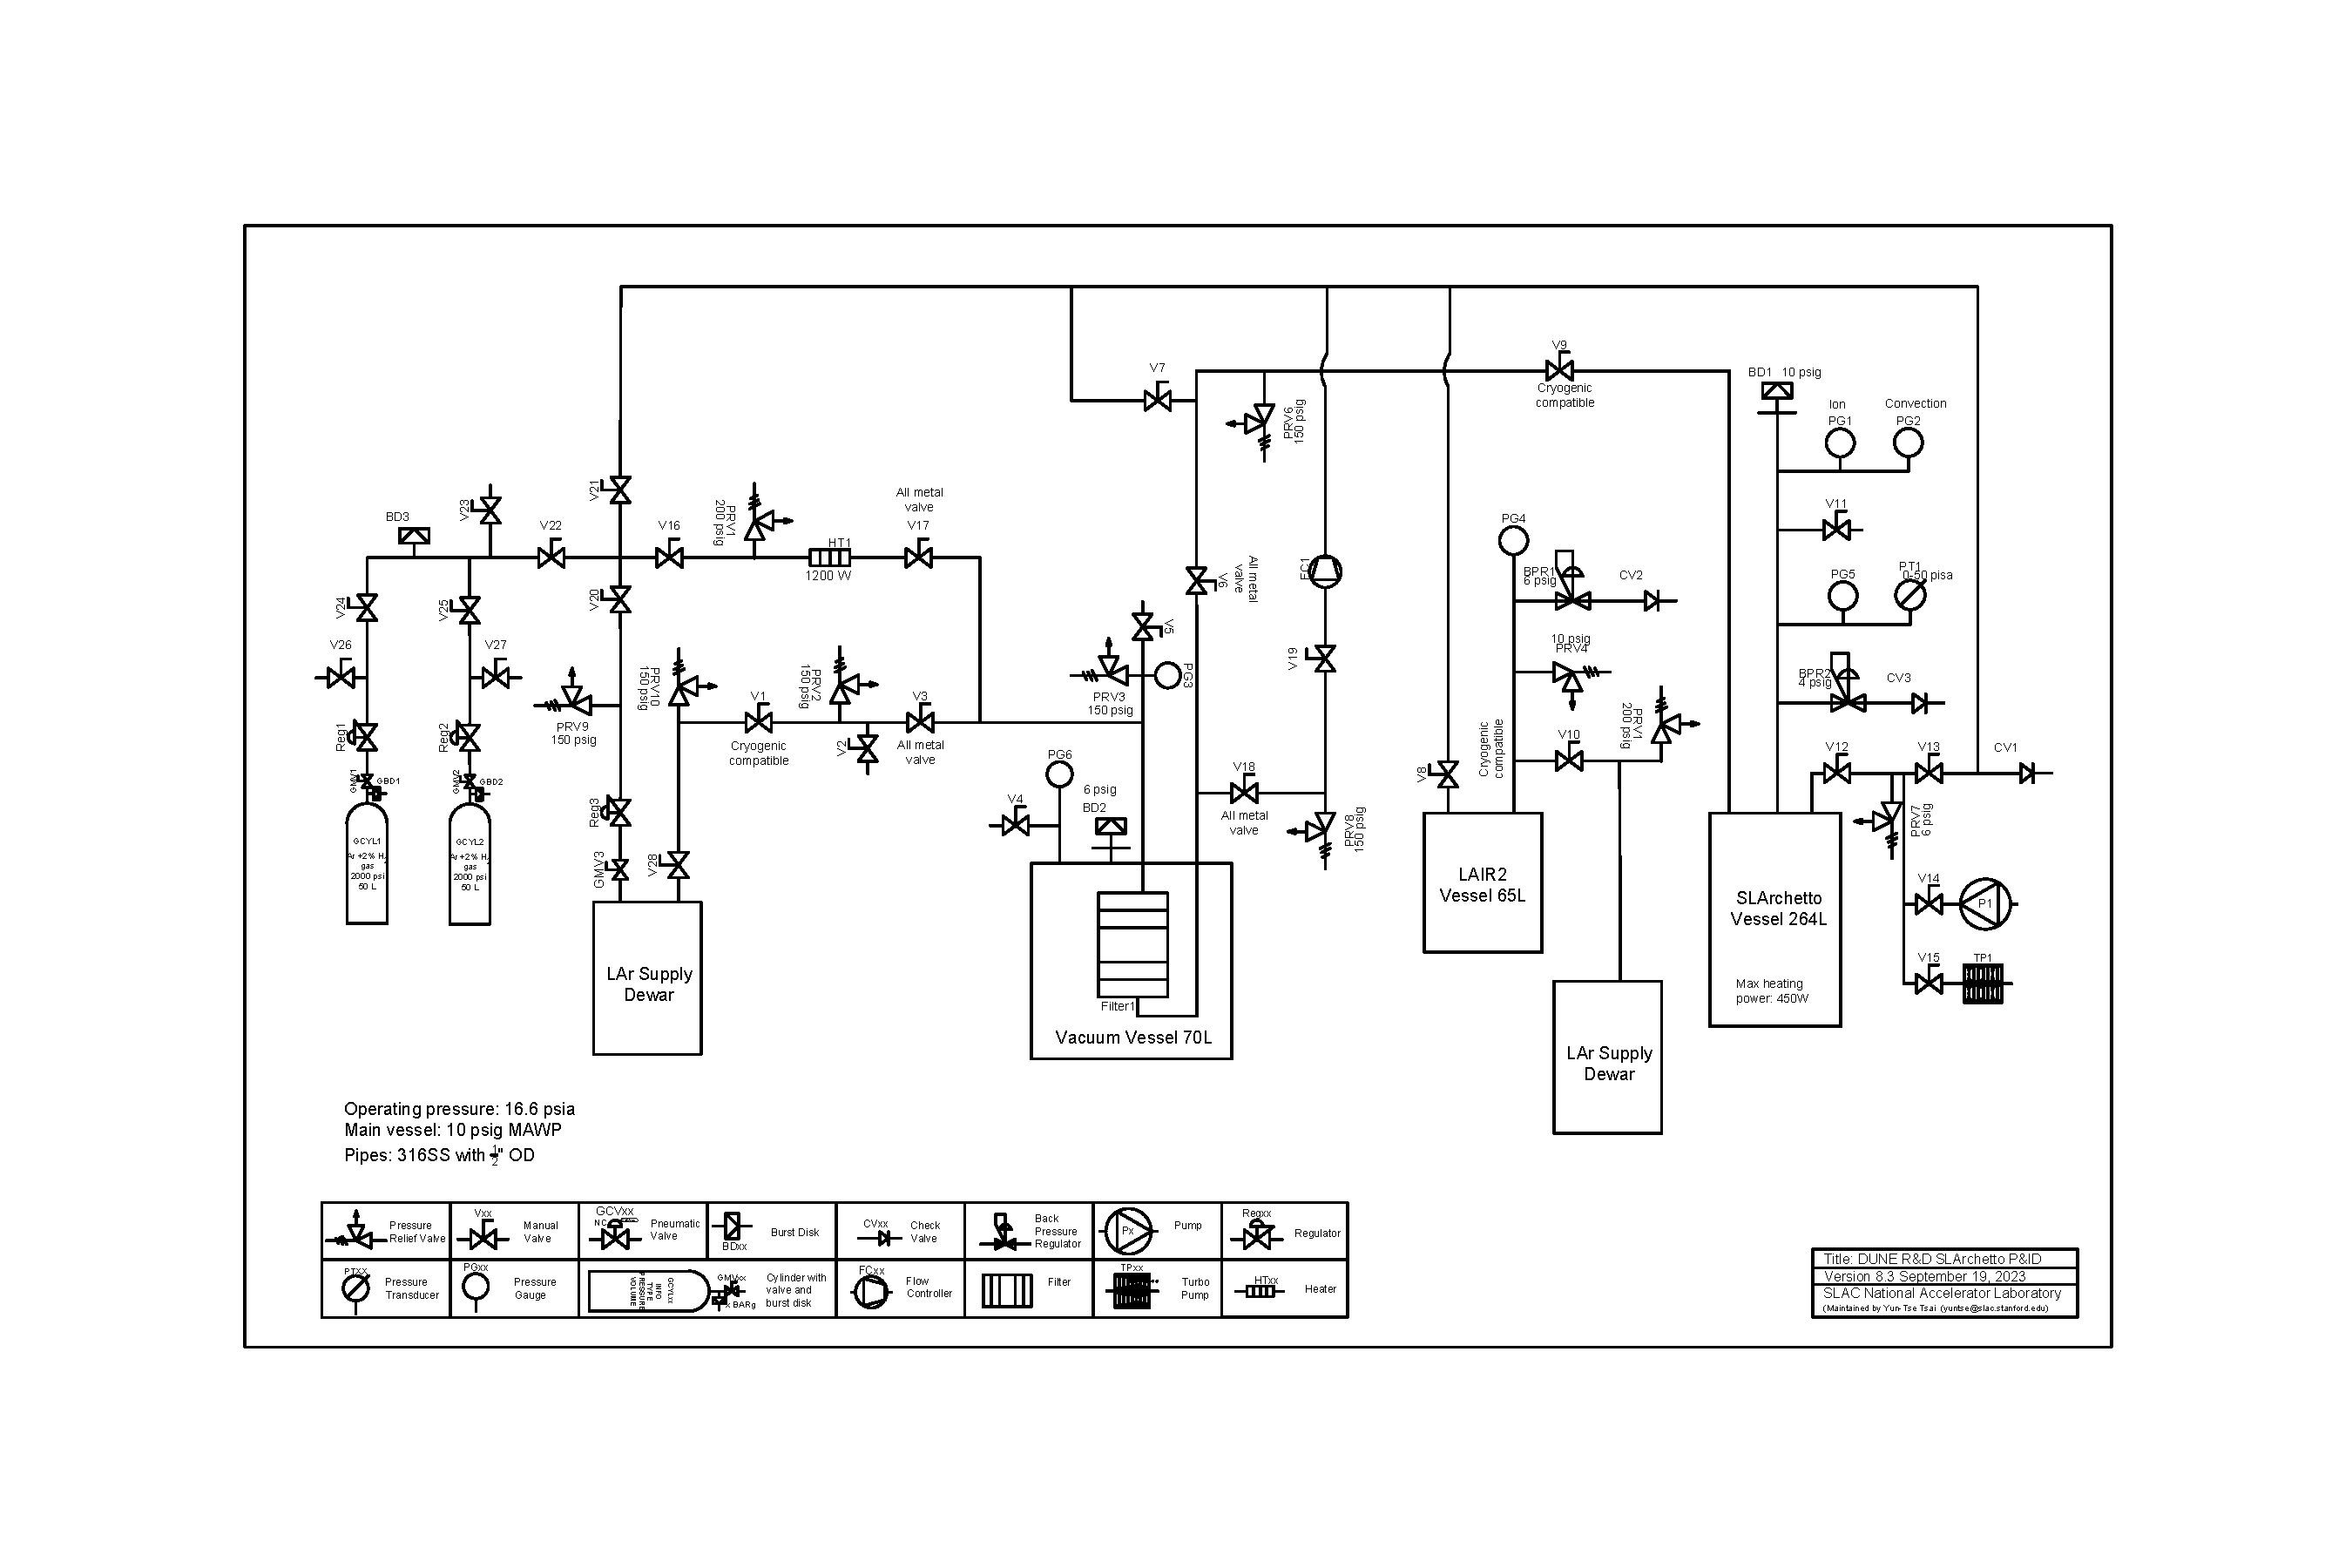
\includegraphics[angle=90,origin=c,height=7.2in]{fig/PIDv8.3.pdf}
\caption{P\&ID}
\end{center}
\end{figure}
%-------------------------------------------------------------------
%-------------------------------------------------------------------
\clearpage
\begin{figure}[htb]
\begin{center}
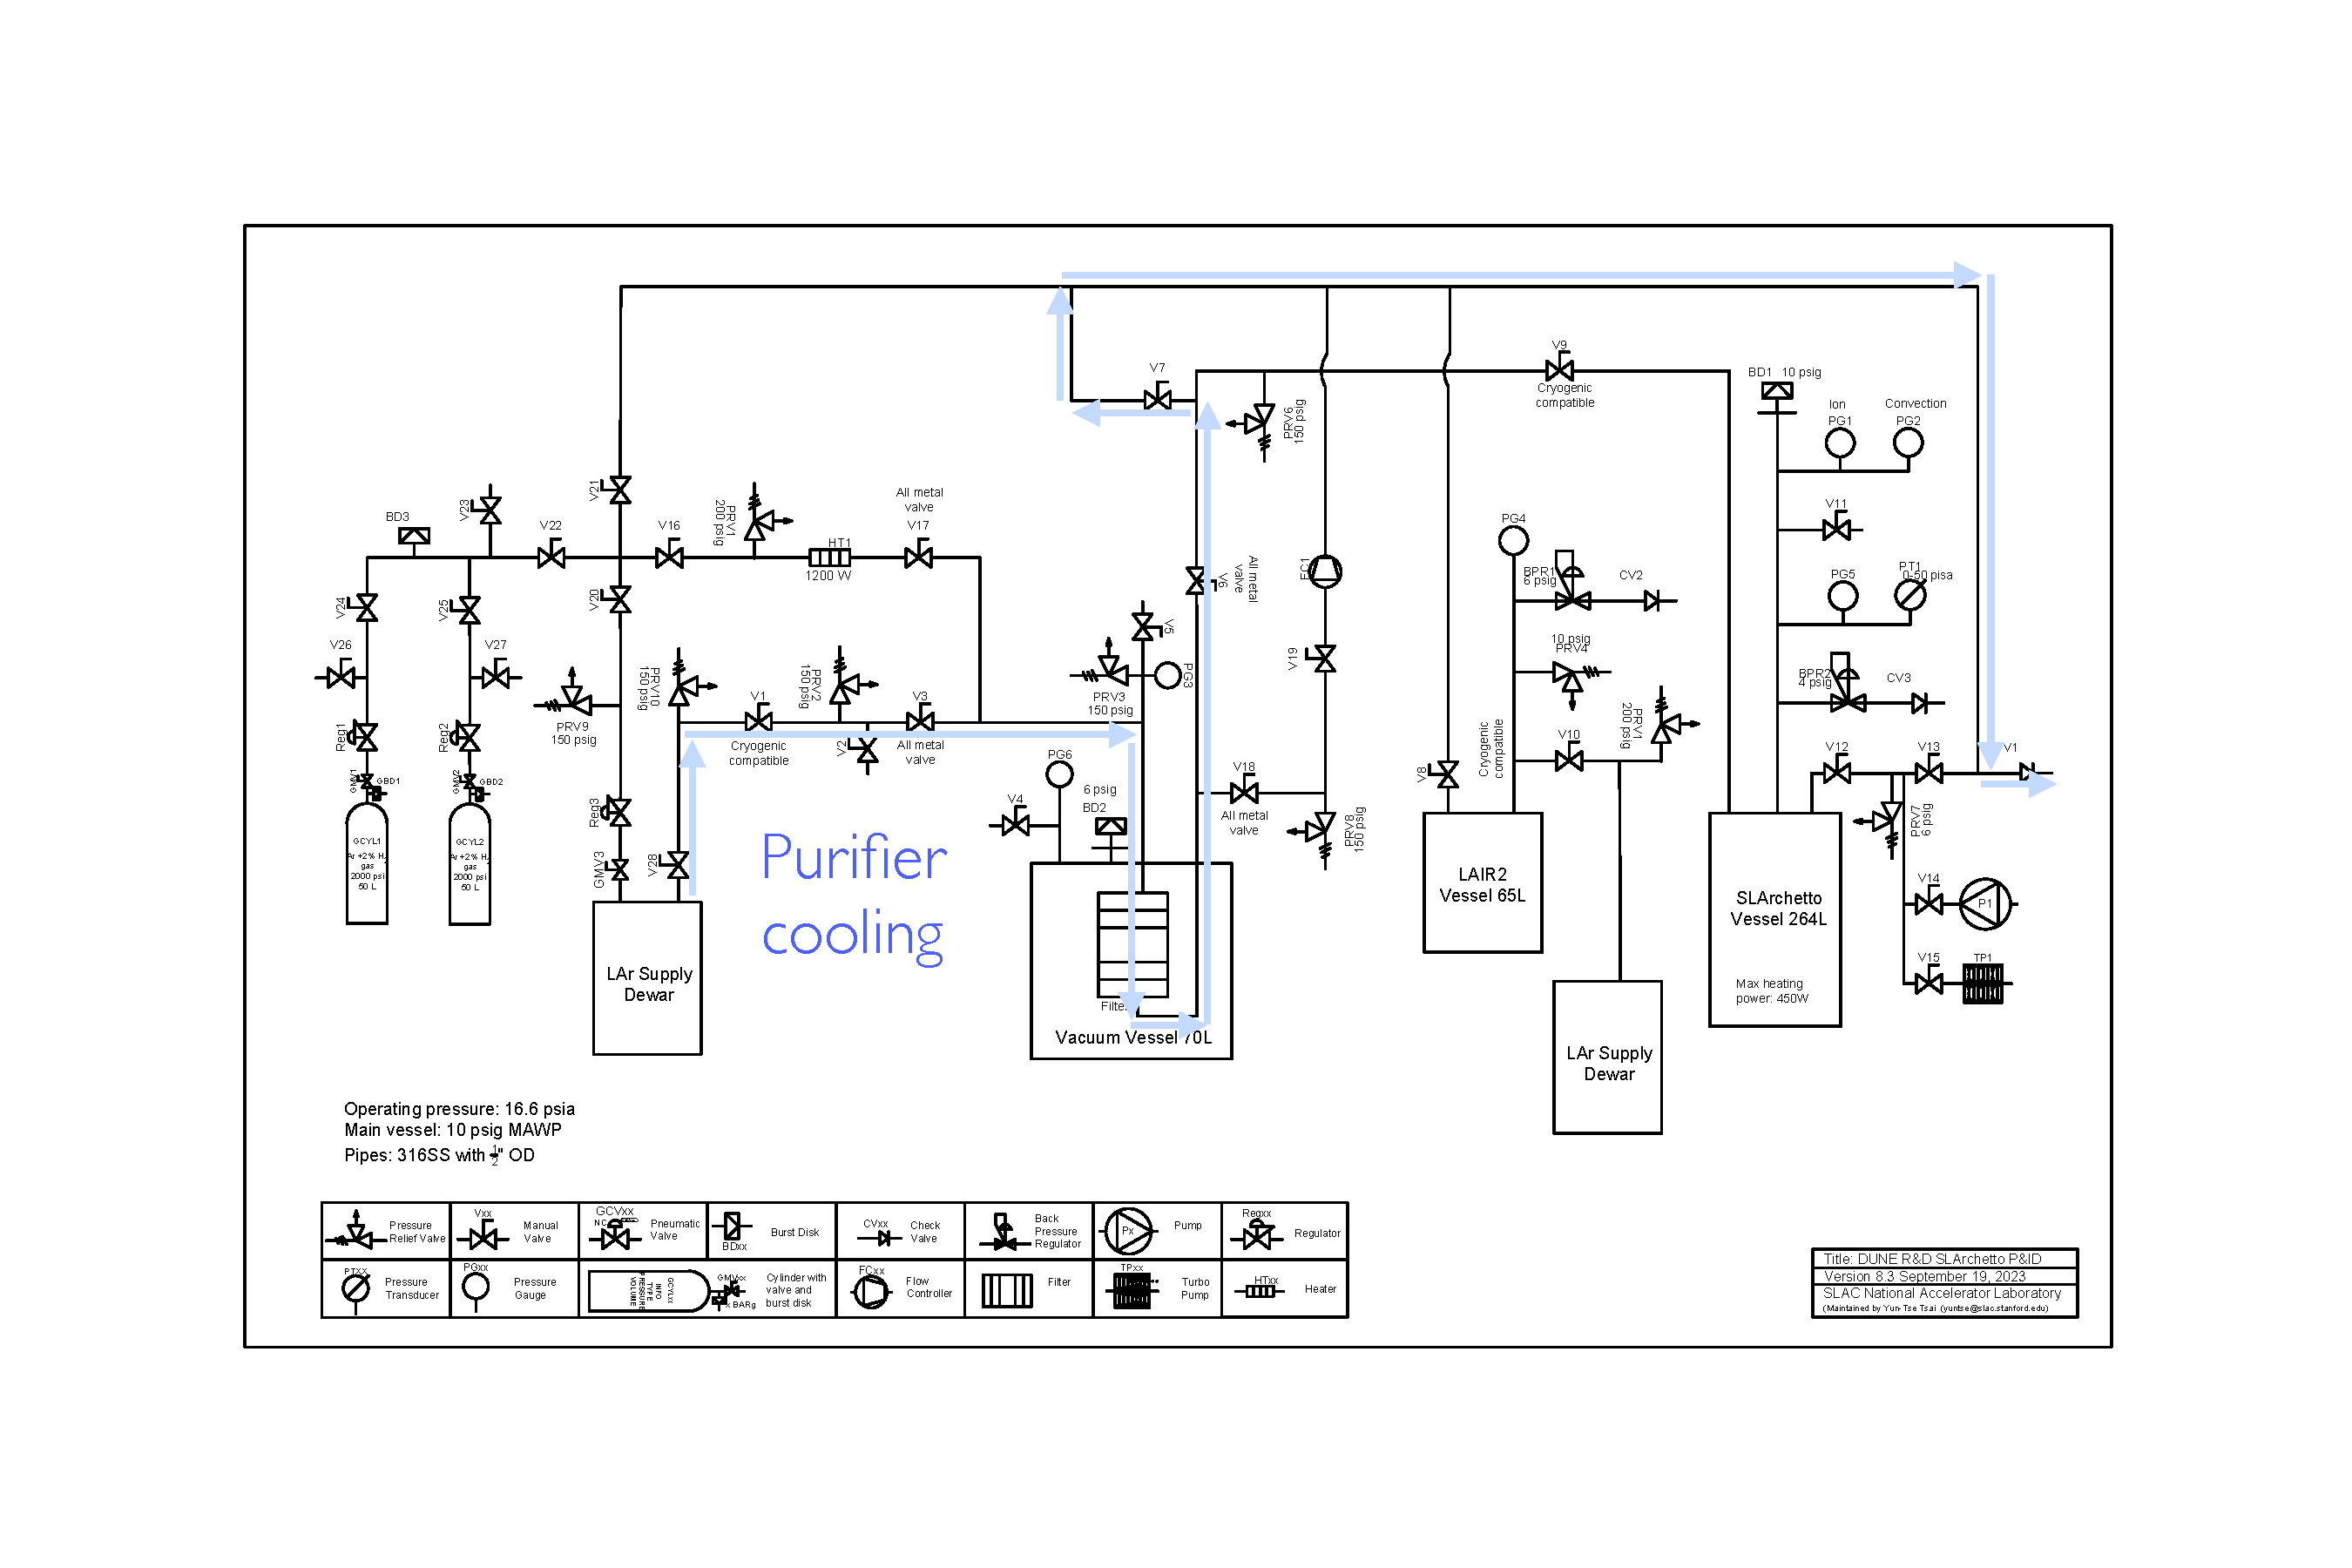
\includegraphics[angle=90,origin=c,height=7.2in]{fig/PurifierCooling_PIDv8.3.pdf}
\caption{LAr flow direction for cooling the LAr purifier}
\end{center}
\end{figure}
%-------------------------------------------------------------------
%-------------------------------------------------------------------
\clearpage
\begin{figure}[htb]
\begin{center}
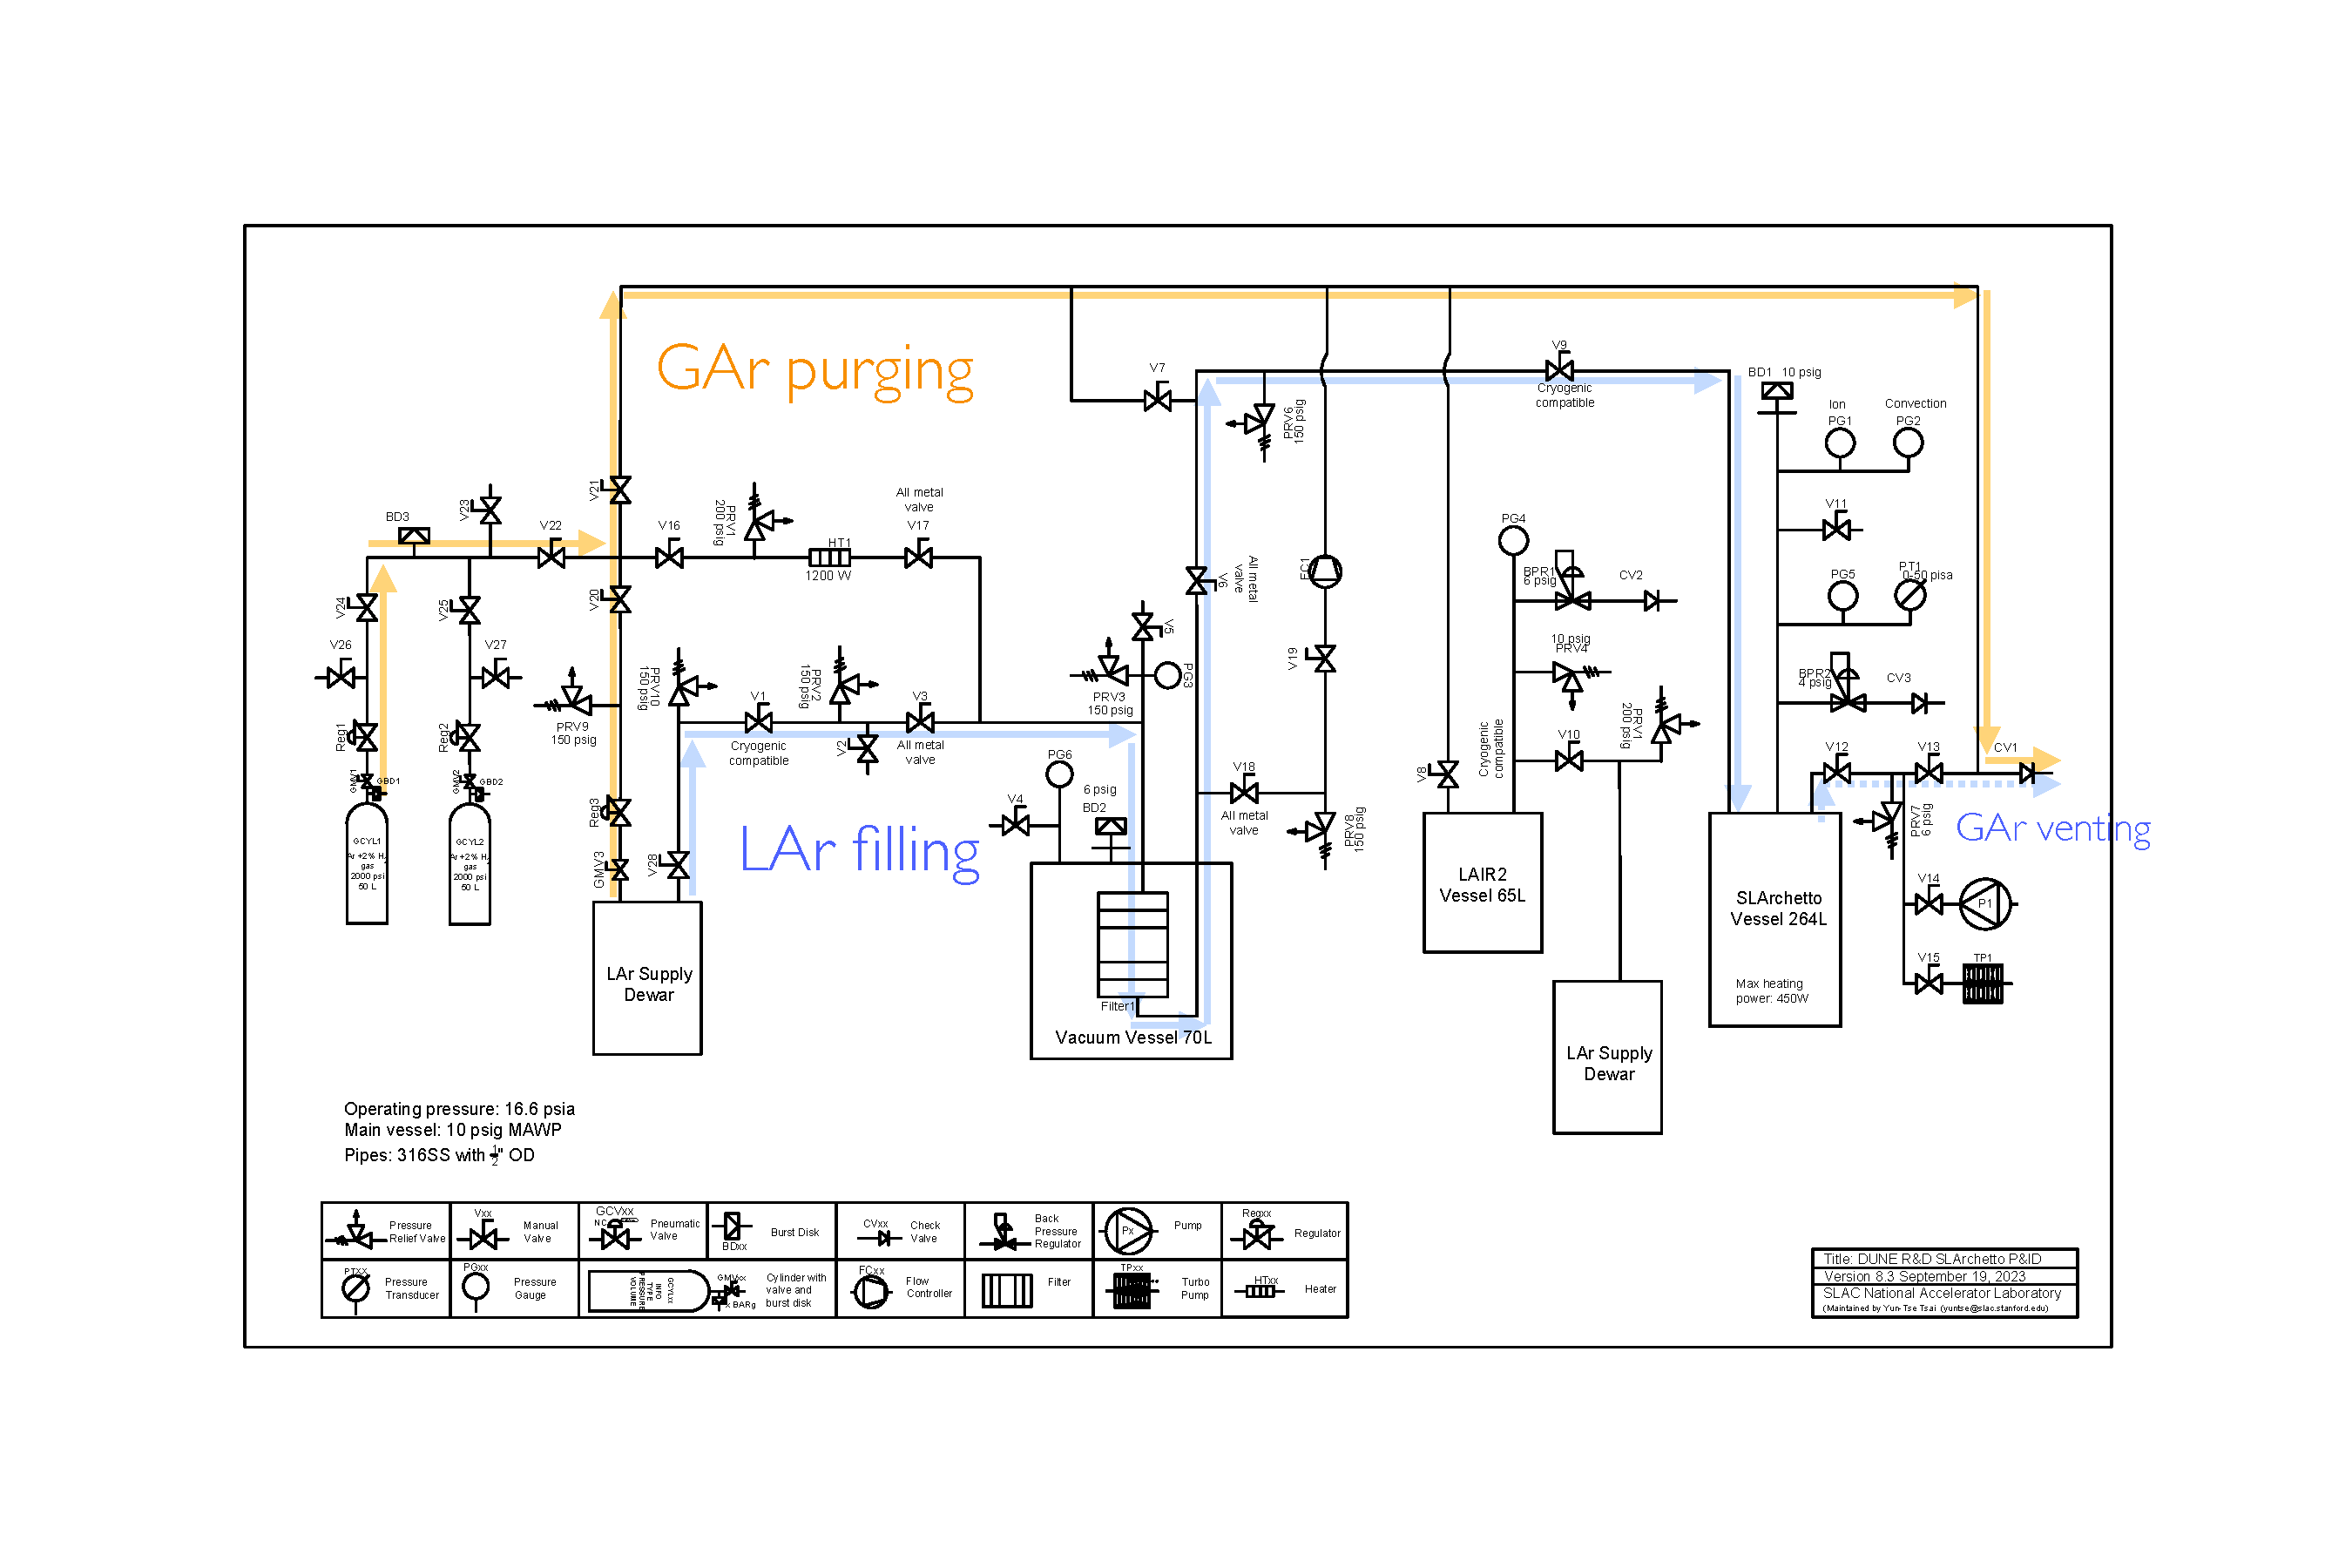
\includegraphics[angle=90,origin=c,height=7.2in]{fig/LArFilling_PIDv8.3.pdf}
\caption{LAr flow direction for filling the SLArchetto vessel.  The gas Ar for purging can be injected from the gas port 
of another LAr dewar, or from an ultra high purity gas argon cylinder.  Do NOT use the same LAr dewar of LAr filling 
for gas Ar purging.}
\end{center}
\end{figure}
%-------------------------------------------------------------------

\clearpage
\tabcolsep=10pt
\begin{longtable}{p{0.5\textwidth}p{0.5\textwidth}}
\hline
\hline
Checklist & What to Do and Detailed Description \\
\hline
\multicolumn{2}{l}{\textbf{Readiness}} \\
\myCheckBox{TPC grounding checked} & \\
\myCheckBox{LArPix tests in the room temperature at atmosphere} & \\
\myCheckBox{Vessel closed and tightened} & \\
\myCheckBox{Leak checked} & \\
\myCheckBox{All valves are closed} &  \\
\myCheckBox{V12, V14 are open} & For pumping the vessel \\
\myCheckBox{P1 (scroll pump) on} & Need to use the scroll pump first \\
\myCheckBox{P1 on for 30 minutes, PG5 (pressure gauge) way below 0 psig, PT1 (pressure transducer) at absolutely 0 
for more than 10 minutes} & Read PT1 from \textbf{Pressure} in the Ignition detector monitor \\
\myCheckBox{V14 closed} & \\
\myCheckBox{P1 off} & \\
\myCheckBox{V15 open} & Prepare to start the turbo pump \\
\myCheckBox{TP1 (turbo pump) on for a few days} &  \\
\myCheckBox{V28 and the valve on the Hicube pump open} & The Hicube pump is located behind the computer monitor.  
V28 is connected on the thermosyphon evaporator, and is not shown in the current version of P\&ID \\
\myCheckBox{The HiCube pump on} & Pump the thermosyphon vacuum jacket \\
\myCheckBox{LAr filter regenerated} & See the procedure for LAr filter regeneration \\
\myCheckBox{Wrap the tubes along the LAr path with foam} & \\
% \myCheckBox{V6, V11, V12 closed, V10 connected to a turbo pump and opened} & Evacuate the tube between V6 and V11/V12 with a turbo pump \\
\myCheckBox{P1 connected to V4.  V4 opened and P1 on} & Evacuate the vacuum vessel insulating the LAr filter \\

\hline
\multicolumn{2}{l}{\textbf{Prepare LAr filling}} \\
\myCheckBox{TP1 (turbo pump) pumped for a few days, PT1  (pressure transducer) at absolutely 0 for a few days, 
ion gauge at $10^{-3}$~mbar} & Read PT1 from \textbf{Pressure} in the Ignition detector monitor.
The ion gauge should be turned off when the pressure is greater than {\color{orange}? mbar} \\
\myCheckBox{The vacuum in the thermosyphon line jacket is at $10^{-3}$ hPa level or below} & 
Read the display at the Hicube pump \\
\myCheckBox{Purge the thermosyphon line} & 
% Open the Tree (botton near home at the top left corner) $\to$ subsystems $\to$ services $\to$ Thermosyphons (we are TSL11).
Use thermosyphon page in DUNE Ignition (button in the main menu or on the thermosyphon temperature panel on the left in the monitor page),
select line TSL11 by clicking on the right thermosyphon or on SLArchetto on the minimap on the top right;
make sure no other valves in the thermosyphon system are being used (large button on the left grey and saying ``No TS valve open''),
so that the control panel and the pressure plot under it are visible and enabled.
\newline Click the top button \texttt{Purge} on the panel.
\newline Purge will take about 3 minutes; while still running the traffic light shows green, turning back off when over.\\

\hline
\multicolumn{2}{l}{\textbf{Safety Checks -- Beginning of the Day}} \\
\myCheckBox{All the doors of the LNTF hut opened} & \\
\myCheckBox{Intake fan on} & Press the red button on the east wall of the LNTF to turn the exhaust 
fan to high speed. Note: Button turns ``yellow'' when the fan is on high speed \\
\myCheckBox{Oxygen deficiency sensor in place, oxygen deficiency monitor green} & \\
\myCheckBox{Ventilation light on} & Red light at the east wall of the LNTF \\
\myCheckBox{Ventilation of the clean room on} & Feel the wind blowing \\
\myCheckBox{HEPAs speed high} & HEPA control is in the back of the fans 
(outside the clean tent), and there are five HEPAs \\

\hline
\multicolumn{2}{l}{\textbf{Cool down the LAr filter}} \\
% \myCheckBox{V2 closed} & \\
\myCheckBox{V15 closed, TP1 (the turbo pump) off} & \\
\myCheckBox{LAr supply dewar has $<$~230 psi} & If it is higher, 
vent the argon to lower pressure $\sim$230 psi.
\newline If it is too low (such as 30 psi), open the pressure builder to 
build the pressure to $>$~100 psi \\
\myCheckBox{Connect the LAr dewar} & \\
% Note that the transfer line between the LAr dewar and V1 is rigid, and we must not overstretch it.  
% Align the connector, and if it is not well aligned, loosen the fitting at V1.  
% If you loosen the fitting at V1, don't forget to change the gasket \\
\myCheckBox{PPE (cryo gloves, safety glasses) on} & \\
% \myCheckBox{LAr supply dewar connected to the transfer line} & \\
\myCheckBox{V1, V2 open} & Purge the air in the tube \\
\myCheckBox{LAr supply dewar (V28) opened} & \\
\myCheckBox{When seeing LAr, V28, V2 closed} & Stop purging \\
\myCheckBox{V6, V3 opened} & \\
\myCheckBox{LAR supply dewar (V28) opened, carefully opened V7 according to PG3} & PG3 should be at 5 -- 10~psig \\
\myCheckBox{Temperature in LAr filter at -100{\dC} (the minimal of the readout device) or cooling for an hour, 
V28 (LAr supply dewar), V7 closed} & \\
% \myCheckBox{Start taking data from the oxygen sensor} & \texttt{miniterm.py --eol=CR 
% --echo /dev/ttyUSB1 | tee 202207xx-01-oxygen.log}, the complete instruction can be found in 
% \href{https://drive.google.com/file/d/1K1IqwLdKXYT1RKmoOM8pu1GDvIFAI1C9/view?usp=sharing}{OxygenSensor.pdf} \\

\hline
\multicolumn{2}{l}{\textbf{Fill the main vessel}} \\
\myCheckBox{Start purging the SLArchetto venting line (downstream V13) with gas Ar} & 
Two options: 1. Use gas Ar from the LAr dewar: Open GMV3, Reg3, V20, V21, 
DO NOT use the same LAr dewar for filling and purging,
2. Use UHP Ar gas cylinder: Hook the gas cylinder, close V26, open GMV1, Reg1, V24, V22, V21\\
\myCheckBox{V15 closed} & \\
\myCheckBox{TP1 (turbo pump) off} & Prepare for filling the main vessel \\
\myCheckBox{LArPix fan on} & Plug the cable into the extension cord used for the turbo pump \\
\myCheckBox{Check V6, V12 open} & \\
\myCheckBox{Double check the closed valves: V2, V5, V7, V8, V9, V11, V13, V14, V15} & \\
\myCheckBox{LAr dewar (V28) closed} & \\
\myCheckBox{Double check the open valves: V1, V3, V6, \textbf{V12 (IMPORTANT)}} & 
V12 is on the top lid, connecting to the hose.  
If closed, the burst disk will crack when LAr just fills in.\\
\myCheckBox{Oxygen sensor shows $<$1\% or plateaued} & Oxygen sensor is displayed at the ``LAr Filter'' 
page of the Ignition GUI \\
\myCheckBox{One operator ready for adjusting V13 all the time according to the pressure in SLArchetto.} &
We want to keep the pressure at about 2~psig at PG5 (16.6~psia at PT1) and not to exceed 
4~psig at PG5 (18.6~psia at PT1) all the time.
We also don’t want the vessel pressure to go below 0~psig at PG5 (14.6~psia at PT1), 
in which condition the air would come in and contaminate the LAr purity. \\
\myCheckBox{The second operator fully opens V9} & \\
\myCheckBox{The second operator opens V28 (LAr dewar) gradually} & \\
% One opens the LAr dewar slightly, and the other monitors PG5 (pressure gauge) or PT1.
% When the pressure reaches 2.5 psig at PG5 (17.1 psia at PT1), open V15 slightly to prevent the pressure from building up.
\myCheckBox{Fill with 10L at 10 slpm, and the pressure is less than 5~bar (better less than 3~bar)} & 
Fill the numbers 10L (large box) at 10 slpm (smaller under the first), and click \texttt{Add N$_2$}.
Check the pressure on the purple graph under the controls.\\
\myCheckBox{LArPix power supply on.  Voltage at 24~V, current limit at 1~A} & \\
\myCheckBox{LArPix starts taking data when the pressure reaches $\sim$14.6~psia} & 
Use \texttt{Pedestal Monitor} in the LArPix tutorial, \url{https://github.com/SLACube/slacube-daq-tutorial}. \\
\myCheckBox{Equilibrium reached and $\sim$50~psig at PG3 (pressure gauge on top of the LAr filter)} & \\
\myCheckBox{Pressure in TSL11 stable and $<$~3~bar, add 5~L at 5~slpm.  Totally 15~L} & \\
\myCheckBox{Pressure in TSL11 stable and $<$~3~bar, add 5~L at 5~slpm.  Totally 20~L} & \\
\myCheckBox{Pressure in TSL11 stable and $<$~3~bar, add 5~L at 5~slpm.  Totally 25~L} & \\
\myCheckBox{Pressure in TSL11 stable and $<$~3~bar, add 5~L at 5~slpm.  Totally 30~L} & \\
\myCheckBox{Pressure in TSL11 stable and $<$~3~bar, add 5~L at 5~slpm.  Totally 35~L} & \\
\myCheckBox{Pressure in TSL11 stable and $<$~3~bar, add 5~L at 5~slpm.  Totally 40~L} & \\
\myCheckBox{Pressure in TSL11 stable and $<$~3~bar, add 5~L at 5~slpm.  Totally 45~L} & \\
\myCheckBox{Pressure in TSL11 stable and $<$~3~bar, add 5~L at 5~slpm.  Totally 50~L} & \\
\myCheckBox{Pressure in TSL11 stable and $<$~3~bar, add 5~L at 5~slpm.  Totally 55~L} & \\
\myCheckBox{Pressure in TSL11 stable and $<$~3~bar, add 5~L at 5~slpm.  Totally 60~L} & \\
\myCheckBox{Pressure in TSL11 stable and $<$~3~bar, add 5~L at 5~slpm.  Totally 65~L} & \\
% \myCheckBox{Pressure in TSL11 stable and $<$~3~bar, add 5~L at 5~slpm.  Totally 70~L} & \\
% \myCheckBox{Pressure in TSL11 stable and $<$~3~bar, add 5~L at 5~slpm.  Totally 75~L} & \\
% \myCheckBox{During fill when the liquid level in the open mouth vessel goes down, open V1 and increase flow to refill} & \\

\hline
\multicolumn{2}{l}{\textbf{LAr dewar transition}} \\
\myCheckBox{When the LAr dewar is almost empty, start to close the LAr dewar} & 
Pressure at PG3 (pressure gauge for the LAr filter) will start dropping when the LAr dewar is almost empty \\
\myCheckBox{1 -- 3~psig at PG5 (pressure gauge for SLArchetto) or 15.6 -- 17.6~psia at PT1 
(pressure transducer for SLArchetto) during the LAr dewar transition} & 
Adjust V13 to control the pressure.  
May need to completely close it.
Read PT1 from \textbf{Pressure} in the Ignition detector monitor \\
\myCheckBox{V1, V3 closed} & \\
\myCheckBox{The first LAr dewar disconnected, the second one connected} & \\
% Note that the transfer line between the LAr dewar and V1 is rigid, and we must not overstretch it.  
% Align the connector, and if it is not well aligned, loosen the fitting at V1.  
% If you loosen the fitting at V1, don't forget to change the gasket \\
\myCheckBox{V1 opened} & \\
\myCheckBox{V28 (LAr dewar), V2 open} & Purge the air in the tube \\
\myCheckBox{When seeing LAr from V2, V28 (LAr dewar), V2 closed} & \\
\myCheckBox{V3 open} & \\
\myCheckBox{Double check V6, V9 opened} & \\
\myCheckBox{One operator ready for adjusting V13 all the time according to the pressure in SLArchetto.} &
We want to keep the pressure at about 2~psig at PG5 (16.6~psia at PT1) and not to exceed 
4~psig at PG5 (18.6~psia at PT1) all the time.
We also don’t want the vessel pressure to go below 0~psig at PG5 (14.6~psia at PT1), 
in which condition the air would come in and contaminate the LAr purity. \\
\myCheckBox{The second operator opens V28 (LAr dewar) gradually} & \\


\hline
\multicolumn{2}{l}{\textbf{Stop LAr filling}} \\
\myCheckBox{Cryocon D (RTD 4) reaches $\sim$90~K at $\sim$16.1~psia, or drops significantly} & 
This means the LAr reaches the desired liquid level.  
Read RTD values at the Ignition detector monitor or the Cryocon device \\
\myCheckBox{Liquid seen through the viewport} & 
Turn on the flash light and place it on top of the viewport shield \\
\myCheckBox{When Cryocan E (RTD 5) shows the beginning of the significant temperature drop, 
two operators ready to close the valves} & \\
\myCheckBox{One operator ready for adjusting V13 all the time according to the pressure in SLArchetto.} &
We want to keep the pressure at about 2~psig at PG5 (16.6~psia at PT1) and not to exceed 
4~psig at PG5 (18.6~psia at PT1) all the time.
We also don’t want the vessel pressure to go below 0~psig at PG5 (14.6~psia at PT1), 
in which condition the air would come in and contaminate the LAr purity. \\
\myCheckBox{V28 (LAr dewar), V13 closed} & \\
\myCheckBox{V1, V3, V6, V9, V12 closed} & \\
\myCheckBox{All valves closed} & \\
\myCheckBox{Stop purging the SLArchetto venting line (downstream V13)} & \\
\myCheckBox{Electrical box plugged and switched on} & 
Toggle up, switch on in case we need heaters \\
\myCheckBox{Set the threshold of LArPix channels with HV off} & 
LArPix DAQ tutorial: \url{https://github.com/SLACube/slacube-daq-tutorial} \\
\myCheckBox{Enable the warning, alert, and alarm for the pressure} & 
Click the alarm button.  Warning range: 14 -- 17.7~psia; Alert range: 14 -- 18.7~psia; 
Alarm range: 14 -- 19.7~psia \\
\myCheckBox{Enable the warning, alert, and alarm for RTD 1, 3, and 4} & 
Click the alarm button.  Warning range: 87 -- 91~K; Alert range: 85 -- 92~K; Alarm range: 83 -- 93~K \\
\myCheckBox{Enable the warning, alert, and alarm for RTD 5} & 
Click the alarm button.  Warning range: 87 -- 130~K; Alert range: 85 -- 130~K; Alarm range: 83 -- 130~K \\
\myCheckBox{Enable the warning and alert for RTD 6} & 
Click the alarm button.  Warning range: 150 -- 163~K; Alert range: 145 -- 170~K \\
% \myCheckBox{Open mouth dewar lowered.  LAr filter warming up.} & Prepare to release the pressure from the LAr evaporation in the LAr filter \\
\myCheckBox{20-40~minutes for equilibrium} & Check for example, if temperature at RTD~4 is rising, if the pressure is stable \\
\myCheckBox{Cryoncon A, B, C, D (RTD 1, 2, 3, 4) show $<$~90K at $\sim$16~psia} & \\
% \myCheckBox{V4, V5, V9, V11, V12 closed.  V6 opened} & Prepare to vent the LAr filter \\
\myCheckBox{LAr filter vented through V5} & \\
\myCheckBox{All valves closed} & 
The valves likely were not closed because of the ice on them.  
Check them again and completely close them \\
\myCheckBox{Emergency exhaust fan button is red} & 
Press the yellow button on the east wall of the LNTF to turn the exhaust fan to low speed. 
Note: Button turns ``red'' when the fan is on low speed \\

\hline
\multicolumn{2}{l}{\textbf{Ramp up high voltage}} \\
\myCheckBox{LArPix data taking stopped} & At this moment, ask Patrick. Will have instructions later \\
\myCheckBox{LArPix tile powered off} & At this moment, ask Patrick. Will have instructions later \\
\myCheckBox{High voltage power supply on} & \\
\myCheckBox{PicoAmmeter on, set to the `zcheck` mode} & \\
\myCheckBox{PicoAmmter DAQ script running and field shell current updating} & Log in
\newline \texttt{neutrino@nu-daq01-ir2.slac.stanford.edu}
\newline run
\newline \texttt{cd \~/kapton\_daq}
\newline \texttt{source setup.sh}
\newline \texttt{nohup python3 daq.py --config config/config\_keithley6485.yaml \&}
\newline Check the \texttt{Current} in the \texttt{HV Control} panel in the main page, 
or \texttt{PicoAm Current} in the \texttt{SLArchetto High Voltage Control} page \\
\myCheckBox{HV status on and HV current set to 1mA} & Go to the \texttt{HV Control} panel, 
and then go to \texttt{HV ramping}.
\newline Click \texttt{PS initialization}.
\newline Then the button \texttt{HV Status On/Off} should be On and green. \\
% \myCheckBox{HV current set to 1mA} & Call Gianluca for testing the new button \\
\myCheckBox{High voltage ramped up to 15~kV} & Set \texttt{Target voltage} to 15~kV, 
and click \texttt{HV ramping Interlock ON}, disabling the interlock.
\newline Click \texttt{Start}.
\newline More details in \href{https://drive.google.com/file/d/1cCuX7aAKU5J-GfdMOtygUpqLafvZ-xzg}{RampingHighVoltage.pdf}. \\
\myCheckBox{High voltage (Cathode voltage) at 15~kV, field shell current (PicoAm Current) 
at $\sim$9000 -- 10000~nA} & Check \texttt{Cathode Voltage} and \texttt{PicoAm Current} in 
the SLArchetto High Voltage Control page, or \texttt{Voltage} and \texttt{Current} in the main monitor \\
\myCheckBox{Enable the alert and alarm for high voltage} & Click the alarm button.  
Warning range: 14.95 -- 15.05~kV; Alert range: 14.9 -- 15.1~kV; Alarm range: 14.8 -- 15.2~kV \\
\myCheckBox{Enable the warning, alert, and alarm for the current} & 
Click the alarm button.  Warning range: -20,000 -- 0~nA; Alert range: -25,000 -- 0~nA; 
Alarm range: -30,000 -- 0~nA \\
\myCheckBox{HV ramping Interlock OFF} & \\

\hline
\multicolumn{2}{l}{\textbf{Start data taking}} \\
\myCheckBox{LArPix tile powered on} & At this moment, ask Patrick. Will have instructions later \\
\myCheckBox{LArPix data taking} & At this moment, ask Patrick. Will have instructions later \\

\hline
\multicolumn{2}{l}{\textbf{Stop operation}} \\
\myCheckBox{Stop data taking} & At this moment, ask Patrick. Will have instructions later \\
\myCheckBox{LArPix tile powered off} & At this moment, ask Patrick. Will have instructions later \\
\myCheckBox{HV and current alarms disabled} & Click the alarm button and disable the alarms \\
\myCheckBox{HV ramped down} & Go to the \texttt{HV Control} panel, and then go to \texttt{HV ramping}.  
Set \texttt{Target voltage} to 0 kV, and click \texttt{HV ramping Interlock ON}, disabling the interlock.  
Click \texttt{Start}.
\newline More details in \href{https://drive.google.com/file/d/1cCuX7aAKU5J-GfdMOtygUpqLafvZ-xzg}{RampingHighVoltage.pdf}. \\
\myCheckBox{High voltage (Cathode voltage) at 0~kV, field shell current (PicoAm Current) at 0~nA} & 
Check \texttt{Cathode Voltage} and \texttt{PicoAm Current} in the SLArchetto High Voltage Control page, 
or \texttt{Voltage} and \texttt{Current} in the main monitor \\
\myCheckBox{HV Status off} & Click \texttt{Switch On}, and the button will become grey and 
\texttt{HV Status Off} will show \\
\myCheckBox{V12 and V13 open} & Prepare for boiling LAr \\
\myCheckBox{Removed liquid nitrogen in the thermosyphon line} 
%% these are instructions before September 2023; still working
% & One way to do so is to remove 1000~L of 
% LN$_2$ at 1~slpm.  It will start pumping and never stop.  Click \texttt{Abort} after a couple of hours, 
% close all the valves and turn off the pump if it is not done automatically.  Then click \texttt{Purge}.\\
& Set the total amount of $N_2$ found in the thermosyphon drawing, e.g.~60~L, to be removed at 1~slpm (click on \texttt{Remove N$_{2}$}).
The script will stop after 4 minutes (i.e.~4 times the expected time),
but when the flux meter at the top of the PID-like drawing shows 0, it's already basically done.
When it's done, click on \texttt{Purge}.\\
\myCheckBox{Heater interlock off} & 
Go to SLArchetto main page, turn off the \texttt{Heater ITLK ON} \\
\myCheckBox{Set up the heater range: 91 -- 95~K} & Go to \texttt{LAr evaporator}, 
set \texttt{Heater OFF temperature} to 95~K while \texttt{Heater ON temperature} to 91~K \\
\myCheckBox{Heater on} & Click \texttt{Start} \\
\myCheckBox{Heat for 24~hours, and heater off} & Go to \texttt{LAr evaporator}, click \texttt{Stop} \\
\myCheckBox{Heater interlock on} & Go to the main page and turn on the heater interlock \\

\hline
\hline
% \caption{}
% \label{}
\end{longtable}



\end{document}
